\section*{Aufgabe 8.2}
In dieser Aufgabe sollte die Dichte in Abhängigkeit der Dichte für verschieden Gittergrößen
geplottet werden. Der Code dafür ist bereits in \lref{bond_perk} dargestellt. Die
resultierenden Kurven sind in \fref{dichte} dargestellt.

\begin{figure}[htb]
  \centering
  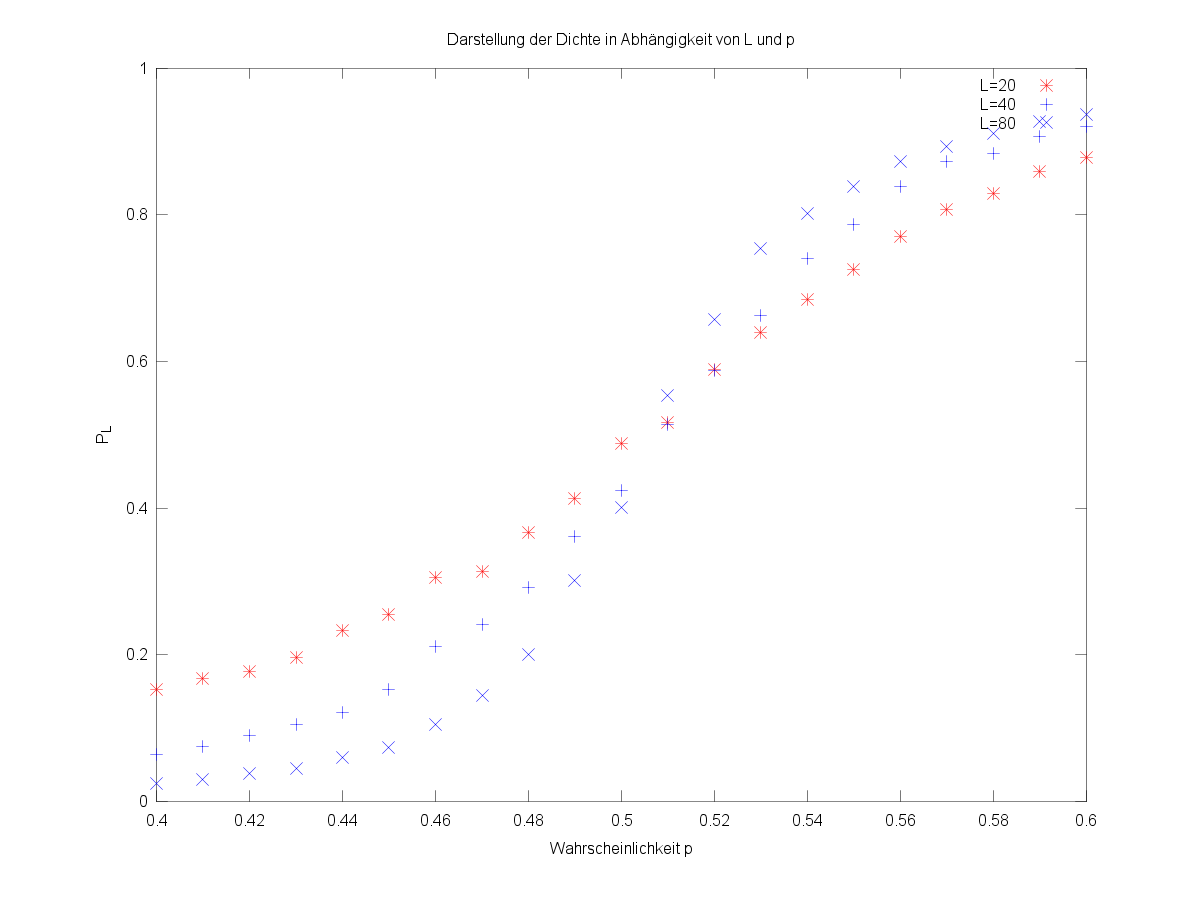
\includegraphics[width=0.8\columnwidth,keepaspectratio]{../tmp/zweitens.png}
  \caption{Dichte in Abhängigkeit von der Wahrscheinlichkeit und für verschiedene Gittergrößen}
  \label{fig:dichte}
\end{figure}

Man erwartet für $p<0.5$, dass die Dichte für sehr große Gitter gegen null geht 
und für größere Wahrscheinlichkeiten gegen 1. Dies kann hier nicht exakt erreicht werden,
da nur endliche Gitter verwendet wurden, aber die entsprechende Tendenz ist erkennbar.
Aufgrund der relativ langwierigen Programmausführung wurde sich auf drei Messwerte beschränkt.